\documentclass{article}
\usepackage[T1]{fontenc}
\usepackage{amssymb, amsmath, graphicx, subfigure, multicol, algorithm, algpseudocode, listings, graphicx}
\graphicspath{ {images/} }

\setlength{\oddsidemargin}{.25in}
\setlength{\evensidemargin}{.25in}
\setlength{\textwidth}{6in}
\setlength{\topmargin}{-0.4in}
\setlength{\textheight}{8.5in}

\newcommand{\heading}[6]{
  \renewcommand{\thepage}{#1-\arabic{page}}
  \noindent
  \begin{center}
  \framebox{
    \vbox{
      \hbox to 5.78in { \textbf{#2} \hfill #3 }
      \vspace{4mm}
      \hbox to 5.78in { {\Large \hfill #6  \hfill} }
      \vspace{2mm}
      \hbox to 5.78in { \textit{Notes By: #4 \hfill #5} }
    }
  }
  \end{center}
  \vspace*{4mm}
}

\newtheorem{theorem}{Theorem}
\newtheorem{definition}[theorem]{Definition}
\newtheorem{remark}[theorem]{Remark}
\newtheorem{lemma}[theorem]{Lemma}
\newtheorem{corollary}[theorem]{Corollary}
\newtheorem{proposition}[theorem]{Proposition}
\newtheorem{claim}[theorem]{Claim}
\newtheorem{observation}[theorem]{Observation}
\newtheorem{fact}[theorem]{Fact}
\newtheorem{assumption}[theorem]{Assumption}

\newenvironment{proof}{\noindent{\bf Proof:} \hspace*{1mm}}{
	\hspace*{\fill} $\Box$ }
\newenvironment{proof_of}[1]{\noindent {\bf Proof of #1:}
	\hspace*{1mm}}{\hspace*{\fill} $\Box$ }
\newenvironment{proof_claim}{\begin{quotation} \noindent}{
	\hspace*{\fill} $\diamond$ \end{quotation}}

\newcommand{\problemset}[3]{\heading{#1}{CS61B: Data Structures}{#2}{Alex Kazorian}{#3}{Section 1: Pointers and Arrays}}



%%%%%%%%%%%%%%%%%%%%%%%%%%%%%%%%%%%%%%%%%%%%%%%%%%%%%%%%%%%%%%%%%%%%%%%%%%%%%%%
% PLEASE MODIFY THESE FIELDS AS APPROPRIATE
\newcommand{\problemsetnum}{1}          % problem set number
\newcommand{\duedate}{\today}
\newcommand{\studentname}{} % problem set deadline
% PUT HERE ANY PACKAGES, MACROS, etc., ADDED BY YOU
%
%%%%%%%%%%%%%%%%%%%%%%%%%%%%%%%%%%%%%%%%%%%%%%%%%%%%%%%%%%%%%%%%%%%%%%%%%%%%%%%
\usepackage{color}

%New colors defined below
\definecolor{codegreen}{rgb}{0,0.6,0}
\definecolor{codered}{RGB}{204,0,0}
\definecolor{codeblue}{RGB}{0,128,255}
\definecolor{backcolour}{rgb}{0.95,0.95,0.92}

%Code listing style named "mystyle"
\lstdefinestyle{mystyle}{
  commentstyle=\color{codegreen},
  keywordstyle=\color{codeblue},
  stringstyle=\color{codegreen},
  basicstyle=\ttfamily,
  breakatwhitespace=false,
  breaklines=true,
  captionpos=b,
  keepspaces=false,
  showspaces=false,
  showstringspaces=false,
  showtabs=false,
  tabsize=2
}

\lstset{style=mystyle}
%%%%%%%%%%%%%%%%%%%%%%%%%%%%%%%%%%%%%%%%%%%%%%%%%%%%%%%%%%%%%%%%%%%%%%%%%%%%%%%
\begin{document}
\problemset{\problemsetnum}{\duedate}{\studentname}

\section*{Overview}

Today's notes will cover various OOP paradigms built into Java. These include inheritance, static and dynamic typing, abstract classes, and interfaces.
Instead of just going a deep conversation about the details of each of these concepts, I feel that it is sufficient to discuss how each of them works. A discussion on why each of these concepts exists and is used will take ages. Everyone has their own opinion in the programming community and we will be here longer than one wants to. Lets get started.

\section{Inheritance}
\begin{lstlisting}[language=Java]
    public class <SubClass> extends <SuperClass> {
        ...
    }
\end{lstlisting}
With this block of code, we introduce three new terms. The description of the terms are as follows:
    \begin{itemize}
        \item \textbf{\textit{extends}}: A keyword that indicates a relationship between two classes.
        \item \textbf{\textit{SubClass}}: A subclass is always to the \textit{left} of the \textit{extends} keyword. The subclass is said to \textit{inherit} from the superclass. This means that the subclass has access to and can use the methods and field attributes of its super class. (There are some cases where this is not true and we will discuss them later!)
        \item \textbf{\textit{SuperClass}}: The superclass is always to the \textit{right} of the \textit{extends} keyword. It is the class being inherited from.
    \end{itemize}
Now, this concept of inheritance gets interesting when we realize that there is nothing restricting a super class from inheriting from another class. This will result in an \textit{inheritance hierarchy} and when designed correctly, these hierarchies give us programmers a lot of power. Do notice that inheritance reinforces and encourages us to be lazy. We don't have to reinvent the wheel. Instead we can inherit from the wheel and make a mode of transport like a bike or car.
\subsection{Some Rules}
The notion of inheritance sounds great, but of course there are some rules attached. They can be summarized as:
    \begin{itemize}
        \item If a class has \textit{final} in its header, then it cannot be extended.
        \item Subclasses cannot access the \textit{private} field attributes and methods of its respective superclass.
        \item The \textit{super} keyword an be used to access field attributes and methods of the superclass if hidden/overridden or call a constructor of the superclass. A hidden field attribute is one that is declared in both the super and sub class.
    \end{itemize}
\newpage
\subsection{Access Modifiers}
\begin{figure}[t]
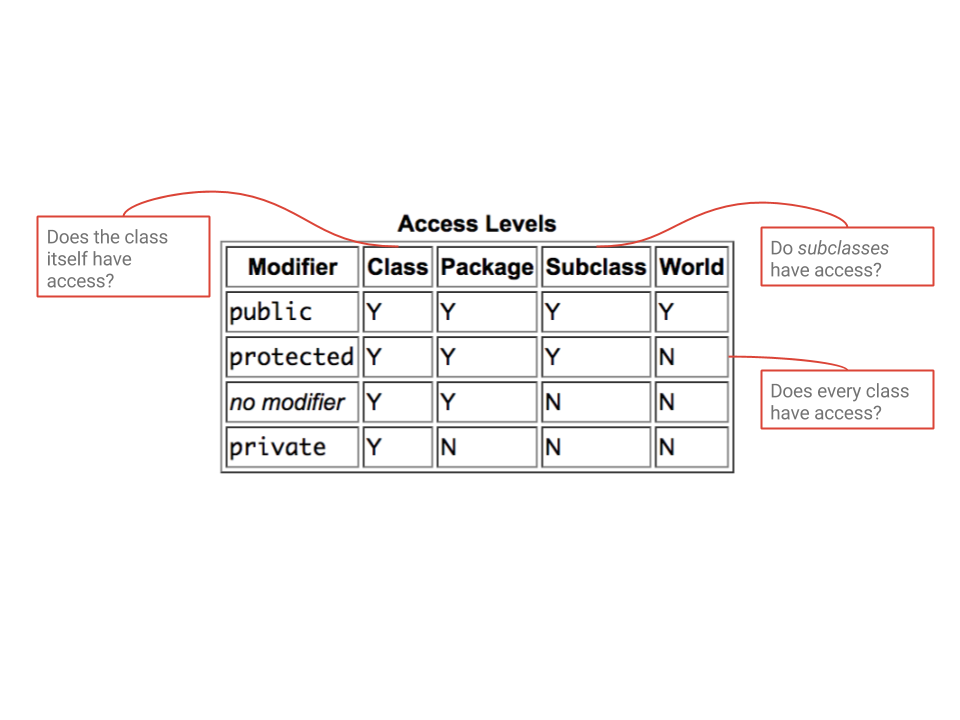
\includegraphics[scale=0.3]{access}
\centering
\end{figure}
Taking a look at the figure above, we have some clarification on the notion of access modifiers and the role they play in inheritance. The idea here is that sometimes, we want to hide data and information from people that do not \textit{need} to use it. Hiding data does not imply that making a field attribute \textit{private} is secure. If only computer security was as simple as making a field attribute \textit{private}!

\section{Polymorphism}
\textit{Polymorphism} is a term that is thrown around a lot right around this time in the course. Simply, it means that an object can be an instance of its respective class, an instance of its superclass, its superclasses superclass, etc... There seems to be some recursive nature to polymorphism, but let us not complicate things. We will keep it simple and consider polymorphism as an "is-a" relationship. In effect, a \textit{subclass} is a \textit{superclass}. More concretely, every \textit{dog} is an \textit{animal}. But, consider the converse of this statement. Is every \textit{animal} a \textit{dog}?
\subsection{Case Study: Dogs and Animals}
Assume the existence of some Animal class and a Dog class that extends from the Animal class. Now consider the following lines of code:
\begin{lstlisting}[language=Java]
    Dog doggo = new Dog();
    Animal doggo = new Dog();
    Dog doggo = new Animal();
\end{lstlisting}
Which of these lines are legal?
\begin{itemize}
    \item Is every \textit{Dog} a \textit{Dog}? Yes.
    \item Is every \textit{Dog} an \textit{Animal}? Yes.
    \item Is every \textit{Animal} a \textit{Dog}? No.
\end{itemize}
Why did I ask these questions? We were trying to declare a new variable in each line. For each of these lines, we tried instantiate an object and claim it \textit{is-an} instance of the variable.
\subsection{Static and Dynamic Types}
Now consider the following line once more:
\begin{lstlisting}[language=Java]
    Dog doggo = new Animal();
\end{lstlisting}
Here the \textit{static} type is \textit{Animal} and the \textit{dynamic} type is \textit{Dog}. We can generalize this statement and say that the \textit{static} type is on the left of the equals sign and the \textit{dynamic} type is on the right. The rule here is that \textit{dynamic} type cannot be a superclass of the \textit{static} type and it must be of the same type or a subclass. \textit{Animal} is a superclass of \textit{Dog} and therefore this is a compilation error. \\ \\
There is an analogy often used to descire the notion of static and dynamic types. We have a box that we try to put dogs in. Any breed of dog can be placed into the box. But if we do not know the type of animal, we cannot confidently say it is a dog; therefore, we are not allowed to place it into the box for dogs. The label on the box is the static type. The type of the animal we are placing into the box is the dynamic type.

% Put bibliography here (if any).
% Example:
%
%\begin{thebibliography}{99}
%
% \bibitem[CLRS]{CLRS}
% Thomas H. Cormen, Charles E. Leiserson, Ronald L. Rivest, and Clifford Stein,
% \emph{Introduction to Algorithms}, Second Edition.
% MIT Press and McGraw-Hill, 2001.
%
%\end{thebibliography}

\end{document}
%%%%%%%%%%%%%%%%%%%%%%%%%%%%%%%%%%%%%%%%%%%%%%%%%%%%%%%%%%%%%%%%%%%%%%%%%%%%%%%
